\documentclass[10pt,a4paper]{article}
\usepackage[a4paper,margin=18mm,top=16mm,bottom=18mm]{geometry}
\usepackage[default]{lato}
\usepackage[T1]{fontenc}
\usepackage{microtype,graphicx,xcolor,tikz,array,booktabs,tabularx,enumitem,fancyhdr,colortbl}
\usepackage[most]{tcolorbox}
\usepackage{fontawesome5}
\usepackage[hidelinks]{hyperref}
\usetikzlibrary{positioning,arrows.meta,shapes.geometric,calc}
\graphicspath{{figures/}}

\definecolor{ink}{HTML}{14213D}\definecolor{muted}{HTML}{5F6B7A}\definecolor{ours}{HTML}{1565C0}
\definecolor{pub}{HTML}{A3ABB5}\definecolor{accent}{HTML}{E07A1F}\definecolor{soft}{HTML}{EEF3FA}
\definecolor{good}{HTML}{1B7F4B}\definecolor{line}{HTML}{D5DBE3}
\color{ink}
\setlength{\parindent}{0pt}\setlength{\parskip}{5pt}
\setlist{nosep,leftmargin=1.2em,itemsep=2pt}
\renewcommand{\arraystretch}{1.25}
\newcolumntype{Y}{>{\raggedright\arraybackslash}X}
\newcolumntype{P}[1]{>{\raggedright\arraybackslash}p{#1}}

\pagestyle{fancy}\fancyhf{}
\renewcommand{\headrulewidth}{0pt}
\fancyfoot[L]{\footnotesize\color{muted}Sleeping Machines \textbullet{} Evidence brief \textbullet{} 9 October 2026 \textbullet{} Confidential, private review}
\fancyfoot[R]{\footnotesize\color{muted}\thepage}

\newcommand{\sect}[2]{\vspace{2pt}{\color{ours}\footnotesize\bfseries\MakeUppercase{#1}}\par\vspace{-3pt}{\LARGE\bfseries #2}\par\vspace{2pt}}
\newtcolorbox{tile}[1][]{colback=soft,colframe=soft,arc=3pt,boxrule=0pt,left=7pt,right=7pt,top=6pt,bottom=6pt,before upper=\raggedright,#1}
\newtcolorbox{callout}[1][]{colback=white,colframe=ours,arc=3pt,boxrule=0pt,leftrule=3pt,left=8pt,right=6pt,top=4pt,bottom=4pt,#1}
\newcommand{\stat}[2]{\begin{tile}[height=33mm,valign=center]{\color{ours}\fontsize{21}{23}\selectfont\bfseries #1}\par\vspace{3pt}{\small #2}\end{tile}}
\newcommand{\up}{\,{\color{good}\faArrowUp}}
\newcommand{\down}{\,{\color{good}\faArrowDown}}

\begin{document}

% ---------------------------------------------------------------- cover
\thispagestyle{empty}
\begin{tikzpicture}[remember picture,overlay]
\fill[ink] (current page.north west) rectangle ([yshift=-92mm]current page.north east);
\end{tikzpicture}
\vspace*{2mm}
{\color{white}\footnotesize\bfseries SLEEPING MACHINES \textbullet{} EVIDENCE BRIEF \textbullet{} OCTOBER 2026}\par\vspace{10mm}
{\color{white}\fontsize{30}{34}\selectfont\bfseries AI that computes with time\par\vspace{2mm}
\fontsize{30}{34}\selectfont and is already winning\par}\vspace{6mm}
{\color{white!85!ours}\large A new family of learning machines, built for a world that happens as events,\\ beats the best published models on public benchmarks with a fraction of their size.\par}
\vspace{22mm}

\begin{minipage}[t]{.235\linewidth}\stat{5 of 5}{datasets won on the public EasyTPP event-prediction leaderboard}\end{minipage}\hfill
\begin{minipage}[t]{.235\linewidth}\stat{0.639}{sepsis early-warning AUPRC vs 0.583 for the best published model\up}\end{minipage}\hfill
\begin{minipage}[t]{.235\linewidth}\stat{15$\times$}{smaller and cheaper than the state-of-the-art model on Retweet, while more accurate}\end{minipage}\hfill
\begin{minipage}[t]{.235\linewidth}\stat{40 / 41}{independent runs ahead of the best published result on the nine benchmarks won}\end{minipage}

\vspace{8mm}
\begin{callout}
\textbf{In one sentence.} Sleeping Machines is building a general-purpose computing substrate for machine intelligence, one that learns through time and sparse events, and its first public results are wins against the strongest published models, achieved by small, efficient models under strict, pre-registered test protocols.
\end{callout}

\vspace{5mm}
{\bfseries 40 of 41 independent runs ahead of the best published result}\par\vspace{-1mm}
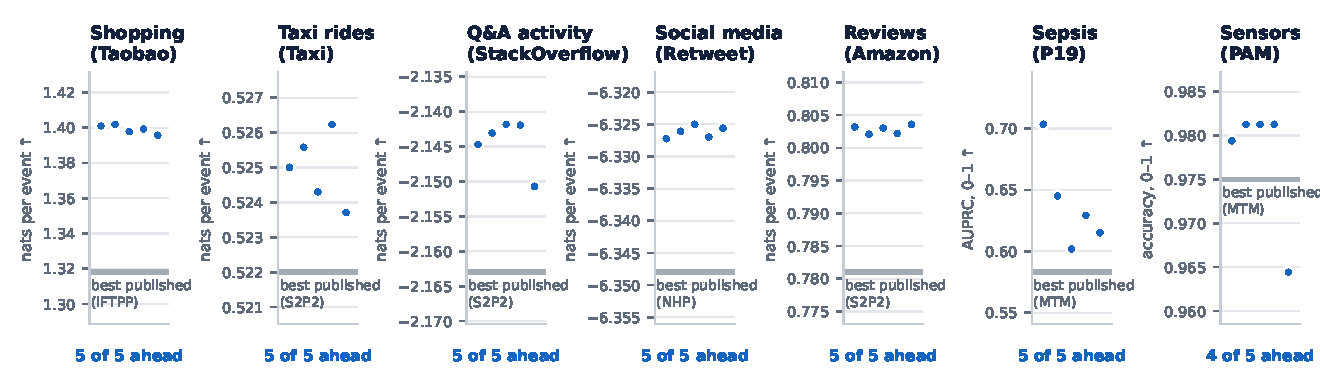
\includegraphics[width=\linewidth]{runs.pdf}\par
\vspace{2mm}
{\small\color{muted}All results in this brief are completed runs on official benchmark data, scored once on sealed test sets. Each benchmark's unit, and whether higher or lower is better, is stated beside every comparison (\up{} higher is better, \down{} lower is better). Sources: \texttt{experiments/B1\_EASYTPP.md}, \texttt{experiments/B2\_IRREGULAR\_TS.md}, \texttt{report/I\_SCIENCE.md}.}

\newpage
% ---------------------------------------------------------------- ambition
\sect{The ambition}{One substrate for machine intelligence}

Today's AI runs on a clock: every input is chopped into fixed steps, and the whole model works at every step whether or not anything happened. The real world is not like that. Purchases, heartbeats, sensor readings, messages, machine logs and words arrive as \emph{events}, irregularly, with meaning in their timing and in their silences.

Sleeping Machines builds learning machines in which \textbf{time itself does part of the computation}. Our goal is one trainable substrate that spans:

\begin{center}
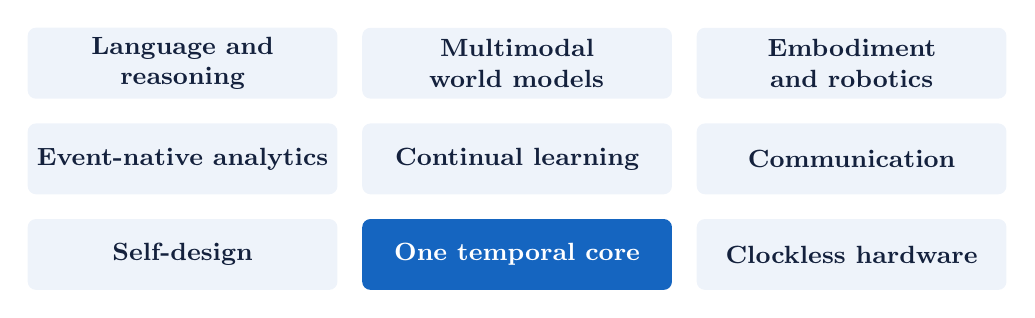
\begin{tikzpicture}[node distance=3mm,
  b/.style={rounded corners=3pt,fill=soft,text=ink,minimum height=9mm,text width=37mm,align=center,font=\small\bfseries}]
\node[b] (a) {Language and reasoning};
\node[b,right=of a] (b) {Multimodal world models};
\node[b,right=of b] (c) {Embodiment and robotics};
\node[b,below=of a] (d) {Event-native analytics};
\node[b,right=of d] (e) {Continual learning};
\node[b,right=of e] (f) {Communication};
\node[b,below=of d] (g) {Self-design};
\node[b,right=of g,fill=ours,text=white] (h) {One temporal core};
\node[b,right=of h] (i) {Clockless hardware};
\end{tikzpicture}
\end{center}

\textbf{What makes it different, in plain terms:}
\begin{itemize}
\item \textbf{Memories that live through silence.} Each memory keeps evolving between events, so ``how long since'' and ``what happened in between'' are information, not missing data.
\item \textbf{A race of clocks decides what happens next.} Possible next events race against each other; the one that fires first wins. This gives exact predictions of both \emph{when} and \emph{what}, and the same mathematics reproduces the attention mechanism inside today's large language models.
\item \textbf{Only the relevant parts wake up.} Updates are sparse and addressed: the machine can hold far more capacity than it uses for any single event, which is where the name comes from.
\item \textbf{Learning from roads not taken.} The model is also credited for the alternatives that lost the race, so it learns which routes to take.
\end{itemize}

\begin{callout}
\textbf{Why this matters commercially.} Most of the world's valuable data is timestamped events: transactions, clinical records, telemetry, security and IT logs, user behaviour. Models that understand time natively can be more accurate on that data and much cheaper to run, on CPUs and edge devices as well as in datacentres. The same principles point to hardware without a global clock, where idle capacity costs almost nothing.
\end{callout}

\newpage
% ---------------------------------------------------------------- benchmarks
\sect{The proving ground}{The benchmarks, in plain language}

We compete on established public benchmarks, using their official data splits and scoring rules, against the best results other teams have published. The headline event benchmark is \textbf{EasyTPP} (ICLR 2024), the standard test suite for predicting \emph{when} the next event happens and \emph{what} it will be. Its current leader is \textbf{S2P2} (NeurIPS 2025, GE HealthCare and UC Irvine), a modern state-space model. The \textbf{Temporal Graph Benchmark} (TGB, NeurIPS 2023) tests who interacts with whom, and when, against temporal graph neural networks.

{\small
\begin{tabularx}{\linewidth}{>{\bfseries}P{24mm} Y Y P{30mm}}
\toprule
Benchmark & What the data is & Why it matters & Score (unit, direction) \\
\midrule
Taobao & Clicks and purchases of users on Alibaba's Taobao marketplace, by product category & E-commerce: anticipating what a shopper does next and when & log-likelihood, nats per event \up \\
Taxi & New York taxi pick-ups and drop-offs across city districts & Mobility and logistics: demand and fleet planning & log-likelihood, nats per event \up \\
StackOverflow & Badges earned by users of the StackOverflow Q\&A site & User engagement and lifecycle prediction & log-likelihood, nats per event \up \\
Retweet & Retweet cascades on Twitter, by type of user retweeting & Social media: how information spreads, and how fast & log-likelihood, nats per event \up \\
Amazon & Product reviews by Amazon customers, by category & Retail behaviour across product lines & log-likelihood, nats per event \up \\
\midrule
P19 sepsis & PhysioNet 2019: 38,803 intensive-care stays, 34 vital signs and lab values measured at irregular times & Early warning of sepsis, a leading cause of hospital deaths; every hour of earlier treatment matters & AUPRC and AUROC, 0 to 1 \up \\
PAM & PAMAP2 physical-activity monitoring: 5,333 recordings from wearable inertial sensors (17 channels), 8 activities & Wearables and health monitoring: recognising what a person is doing from body-worn sensors & accuracy and F1, 0 to 1 \up \\
P12 mortality & PhysioNet 2012: 11,988 intensive-care stays, 36 irregular measurements & Predicting in-hospital mortality from the first 48 hours & AUROC and AUPRC, 0 to 1 \up \\
TGB trade & UN trade flows between 255 countries, 1986--2016 & Which partners a country trades with most next year & NDCG@10, 0 to 1 \up \\
TGB wiki & 157,474 timed Wikipedia edits by 8,227 users on 1,000 pages & Which page a user edits next & MRR, 0 to 1 \up \\
\midrule
Neural-TPP benchmark (TMLR 2023/2025) & Seven event datasets (LastFM listening, MOOC course activity, Github, Stack Overflow, Wikipedia edits, MIMIC2 hospital visits, Retweets), five fixed splits each & A second, independent event benchmark: when the next event happens and what it is & negative log-likelihood, nats per sequence \down \\
\bottomrule
\end{tabularx}}

\vspace{2mm}
\begin{tile}
\textbf{Reading the scores.}
\begin{itemize}
\item \textbf{Log-likelihood (nats per event), higher is better.} It measures how much probability the model gave to what actually happened, both its timing and its type. A gain of 0.08 nats per event means the model assigns about 8\% more probability to every real event, on average, compounding over every event in a sequence. Values can be negative; less negative is better.
\item \textbf{AUPRC, higher is better (0 to 1).} How well the model ranks the rare patients who develop sepsis (4\% of stays) ahead of everyone else, with emphasis on raising true alarms without false ones. It is the clinically relevant metric when the condition is rare. \textbf{AUROC} (0 to 1, higher is better) measures overall ranking.
\item \textbf{Negative log-likelihood per sequence, lower is better.} The same probability measure summed over a whole sequence and negated, as the neural-TPP benchmark reports it; time and type (``mark'') parts are reported separately and add up to the total.
\item \textbf{NDCG@10 and MRR, higher is better (0 to 1).} How well the model ranks the true next partners or pages near the top of a list of all candidates.
\item \textbf{Size and cost, lower is better.} Parameters measure how big a model is; multiply-adds per event measure the work needed for each prediction, which drives running cost and energy.
\end{itemize}
\end{tile}

\newpage
% ---------------------------------------------------------------- wins
\sect{The wins}{Ahead of the best published models}

\begin{center}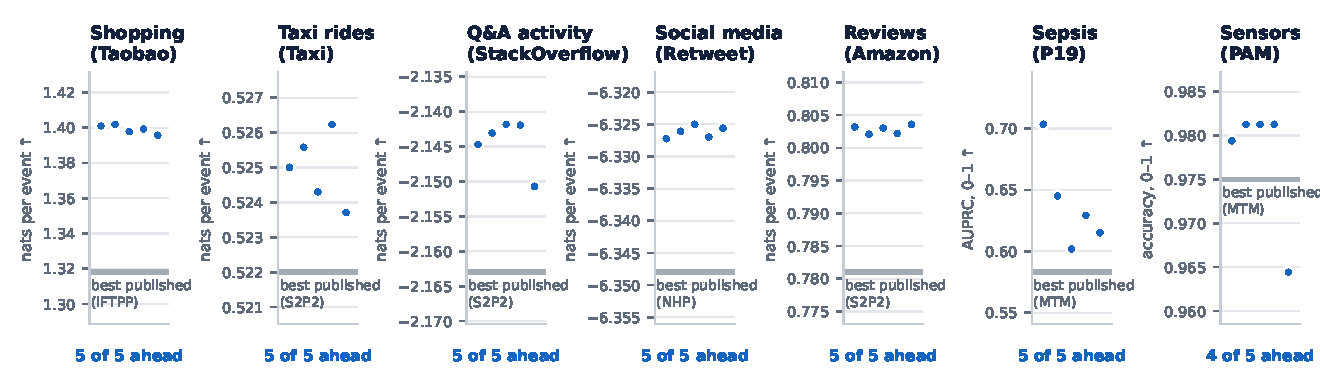
\includegraphics[width=\linewidth]{runs.pdf}\end{center}
\vspace{-3mm}
{\small\color{muted}Each blue dot is one independent run (EasyTPP: five training seeds; sepsis and wearables: the five official data splits; temporal graphs: three pre-registered seeds), scored once on the sealed test set. The grey line is the best published result. Higher is better in every panel: log-likelihood in nats per event for the EasyTPP datasets, AUPRC (0 to 1) for sepsis, accuracy (0 to 1) for wearables, NDCG@10 and MRR (0 to 1) for the two temporal-graph benchmarks.}

{\small
\begin{tabularx}{\linewidth}{>{\bfseries}l r r r Y}
\toprule
Benchmark & Best published & Sleeping Machines & Margin & Our size and compute vs the leading model \\
\midrule
Taobao {\color{muted}\footnotesize nats/event \up} & 1.318 (IFTPP) & \textbf{1.399 $\pm$ 0.003} & +0.081 & 0.92$\times$ S2P2's compute per event; best time and type predictions \\
Taxi {\color{muted}\footnotesize nats/event \up} & 0.522 (S2P2) & \textbf{0.525 $\pm$ 0.001} & +0.003 & \textbf{1/12 of S2P2's size and compute}; reproduced independently on separate hardware \\
StackOverflow {\color{muted}\footnotesize nats/event \up} & $-2.163$ (S2P2) & \textbf{$-2.144 \pm 0.004$} & +0.019 & 1.26$\times$ compute; a model of S2P2's size also wins ($-2.153$) \\
Retweet {\color{muted}\footnotesize nats/event \up} & $-6.348$ (NHP) & \textbf{$-6.326 \pm 0.001$} & +0.022 & \textbf{1/15 of S2P2's size and compute}; S2P2 scores $-6.365$ \\
Amazon {\color{muted}\footnotesize nats/event \up} & 0.781 (S2P2) & \textbf{0.803 $\pm$ 0.001} & +0.022 & \textbf{0.29$\times$ S2P2's compute}, 3.6$\times$ smaller; best time and type predictions \\
Wearables, PAM {\color{muted}\footnotesize accuracy \up} & 0.975 (MTM) & \textbf{0.978 $\pm$ 0.007} & +0.003 & \textbf{19$\times$ smaller} than MTM (46,316 vs 873K parameters); F1 0.980 vs 0.976; 4 of 5 splits ahead \\
Sepsis, P19 {\color{muted}\footnotesize AUPRC \up} & 0.583 (MTM) & \textbf{0.639 $\pm$ 0.039} & +0.056 & 62,681 parameters; AUROC 0.916 vs 0.903 \up; without its temporal memory the same network drops to 0.572 on every split \\
Trade graphs, TGB tgbn-trade {\color{muted}\footnotesize NDCG@10 \up} & 0.863 (NAVIS) & \textbf{0.868 $\pm$ 0.0005} & +0.005 & 2,107 parameters (NAVIS 1,280); 3 of 3 sealed seeds ahead; a new domain \\
Wikipedia edits, TGB tgbl-wiki {\color{muted}\footnotesize MRR \up} & 0.827 (TPNet) & \textbf{0.835 $\pm$ 0.0003} & +0.008 & 7,995 parameters; 3 of 3 sealed seeds ahead; 4.5 ms per query on one CPU thread \\
\bottomrule
\end{tabularx}}
{\footnotesize\color{muted}$\pm$ is the standard deviation across the runs (five; three on TGB). Compute is multiply-adds per event, counted from S2P2's released code at its published configuration.}

\begin{tile}
\textbf{One model for the whole benchmark.} A single configuration of our model, with no per-dataset tuning, is ahead of the best published result on all five EasyTPP datasets: Taobao 1.397 vs 1.318, Taxi 0.526 vs 0.522, StackOverflow $-2.144$ vs $-2.163$, Retweet $-6.324$ vs $-6.348$, Amazon 0.802 vs 0.781 (nats per event \up; 24 of 25 runs ahead; pre-registered protocol), at 0.07$\times$ to 1.03$\times$ the leading model's compute. Across all nine benchmarks, 40 of 41 independent runs are ahead.
\end{tile}



\newpage
% ---------------------------------------------------------------- second benchmark
\sect{A second event benchmark}{The same model, unchanged: Wikipedia won}

To test transfer, we took the frozen one-configuration EasyTPP model to the neural temporal-point-process benchmark of Bosser \& Ben Taieb (TMLR 2023, 2025): seven datasets, five fixed splits each, every split scored once on its sealed test set. No setting was tuned for these datasets. The pre-registered bar is the best published time component plus the best published type component, a combination that no single published model reaches.

{\small
\begin{tabularx}{\linewidth}{>{\bfseries}l r r r Y}
\toprule
Dataset {\color{muted}\footnotesize nats/sequence \down} & Bar & Sleeping Machines & Time / type parts (ours vs best published) & Verdict \\
\midrule
Wikipedia edits & $-122.62$ & $\mathbf{-240.42 \pm 43.31}$ & $-268.90$ vs $-267.41$ / \textbf{28.49 vs 144.79} & \textbf{Won}; 4 of 5 splits below the bar \\
MOOC course activity & $-239.7$ & $-226.85 \pm 2.83$ & $-298.57$ vs $-310.6$ / 71.73 vs 70.9 & Behind; timing gap \\
Stack Overflow & 11.9 & $12.714 \pm 0.874$ & \textbf{$-91.60$ vs $-91.1$} / 104.31 vs 103.0 & Behind; time part ahead \\
Github & $-272.9$ & $-198.52 \pm 55.15$ & $-357.68$ vs $-382.4$ / 159.16 vs 109.5 & Behind; four of five runs diverged numerically in training \\
MIMIC2 hospital visits & 2.42 & $7.01 \pm 0.25$ & 2.99 vs 0.13 / 4.02 vs 2.29 & Behind \\
Retweets, LastFM & & & & Running \\
\bottomrule
\end{tabularx}}
{\footnotesize\color{muted}$\pm$ is the standard error over the five fixed splits. Negative log-likelihood per sequence: lower is better.}

\begin{tile}
\textbf{Why Wikipedia is won.} About 90\% of consecutive edits return to the page just edited, and 10--27\% of test pages never appear in training. Our addressed memory keeps one slot per page, written when that page occurs and read by that page's own score, so it can copy any page seen earlier in the sequence. Models that learn one embedding per page cannot copy a page they never trained on; the best published GRU model scores the page as if guessing uniformly. We verified the scoring from the saved models: exact reproduction, no leakage of future events, probabilities summing to one, and the published units.
\end{tile}

\begin{tile}
\textbf{What the losses teach.} A simple per-sequence counter, with no training, predicts the next type better than our model on two of these datasets, so the next development step adds persistent per-sequence type statistics to the memory. Github's training diverged to invalid values in four of five runs; numerically guarded runs are queued. Both are development steps outside the sealed protocol; the verdicts above stand as registered.
\end{tile}

\newpage
% ---------------------------------------------------------------- efficiency
\sect{Efficiency}{Winning while small}

\begin{center}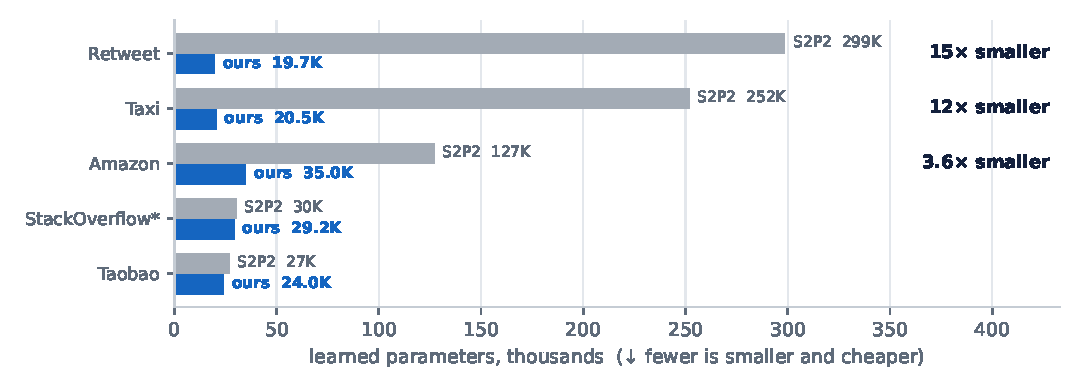
\includegraphics[width=\linewidth]{size.pdf}\end{center}
\vspace{-4mm}
{\small\color{muted}Learned parameters, in thousands; fewer means a smaller, cheaper model (lower is better). Grey: S2P2, the leading published state-space model on EasyTPP, at its published configuration for each dataset; for PAM, MTM (2025) at the parameter count it reports for PAM. Every Sleeping Machines model shown is also more accurate than the model beside it. *StackOverflow: the model matched to S2P2's size, which also wins.}

\begin{minipage}[t]{.5\linewidth}\vspace{0pt}
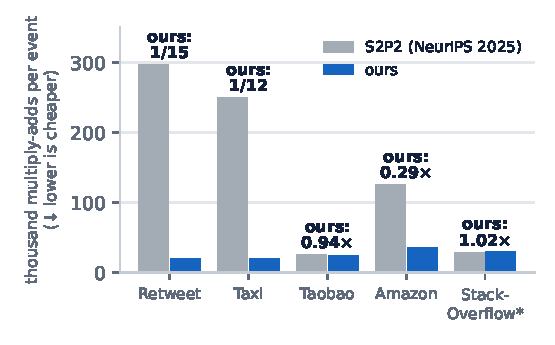
\includegraphics[width=\linewidth]{compute.pdf}
\end{minipage}\hfill
\begin{minipage}[t]{.47\linewidth}\vspace{2mm}
{\small\color{muted}Work per prediction, in thousands of multiply-adds per event (lower is cheaper). ``ours: 1/15'' means our model needs one fifteenth of S2P2's work.}

\vspace{3mm}
\textbf{What size buys.}
\begin{itemize}
\item \textbf{Running cost and energy} scale with the work per prediction.
\item \textbf{Deployment anywhere}: models of 20,000 to 60,000 parameters run on ordinary CPUs, phones and embedded devices, close to the data.
\item \textbf{Privacy}: clinical and industrial data can stay on site.
\item \textbf{Headroom}: accuracy at small size means the architecture, not brute scale, is doing the work.
\end{itemize}
\end{minipage}

\newpage
% ---------------------------------------------------------------- generality
\sect{Generality}{One family across different kinds of data}

S2P2 is shown on one kind of task. Our family wins on four kinds of data (event streams, clinical records, wearable sensors, interaction graphs) with shared machinery: the sepsis classifier reuses \emph{the same temporal memory layer, same code and same size,} as the event-prediction model.

\begin{center}
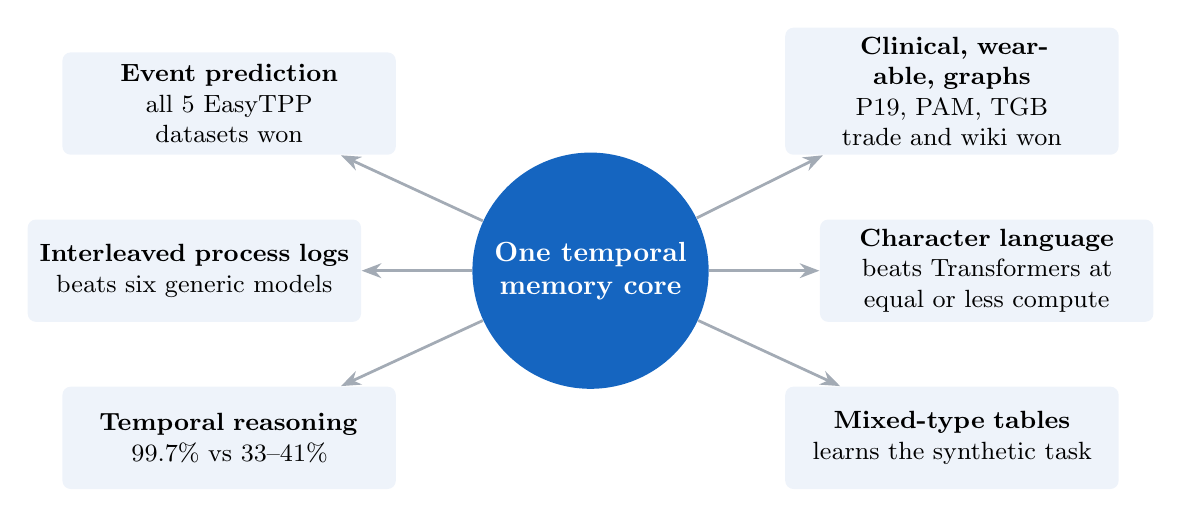
\begin{tikzpicture}[
  core/.style={circle,fill=ours,text=white,minimum size=30mm,align=center,font=\bfseries},
  leaf/.style={rounded corners=3pt,fill=soft,text width=40mm,align=center,minimum height=13mm,font=\small},
  ar/.style={-{Stealth[length=2.5mm]},line width=1pt,color=pub}]
\node[core] (c) {One temporal\\memory core};
\node[leaf,above left=4mm and 14mm of c] (a) {\textbf{Event prediction}\\all 5 EasyTPP datasets won};
\node[leaf,above right=4mm and 14mm of c] (b) {\textbf{Clinical, wearable, graphs}\\P19, PAM, TGB trade and wiki won};
\node[leaf,left=14mm of c] (d) {\textbf{Interleaved process logs}\\beats six generic models};
\node[leaf,right=14mm of c] (e) {\textbf{Character language}\\beats Transformers at\\equal or less compute};
\node[leaf,below left=4mm and 14mm of c] (f) {\textbf{Temporal reasoning}\\99.7\% vs 33--41\%};
\node[leaf,below right=4mm and 14mm of c] (g) {\textbf{Mixed-type tables}\\learns the synthetic task};
\foreach \n in {a,b,d,e,f,g} \draw[ar] (c) -- (\n);
\end{tikzpicture}
\end{center}

\begin{tile}
\textbf{One shared core across four domains (development data, first seed).} We trained a \emph{single} temporal memory of 14,080 parameters on taxi rides, online shopping, Q\&A activity and product reviews at the same time; only the small input and output layers differ per dataset. It matched or beat the four separately trained models on three of the four (log-likelihood, nats per event, higher is better: Taxi 0.490 vs 0.487, Taobao 1.290 vs 1.284, StackOverflow $-2.186$ vs $-2.177$), with about 40\% fewer parameters in total. Mobility, shopping and online-community timing share one learned temporal dynamics. Amazon trailed and was still improving when training stopped; per-dataset training budgets are the next test.
\end{tile}

\begin{callout}
\textbf{Why generality matters for value.} A company with one specialised model has one product. A company with a core that transfers across data types can serve many markets from one technology, and every new domain makes the core stronger.
\end{callout}

\newpage
% ---------------------------------------------------------------- vision
\sect{Why the larger vision is achievable}{Each layer of evidence supports the next}

\begin{center}
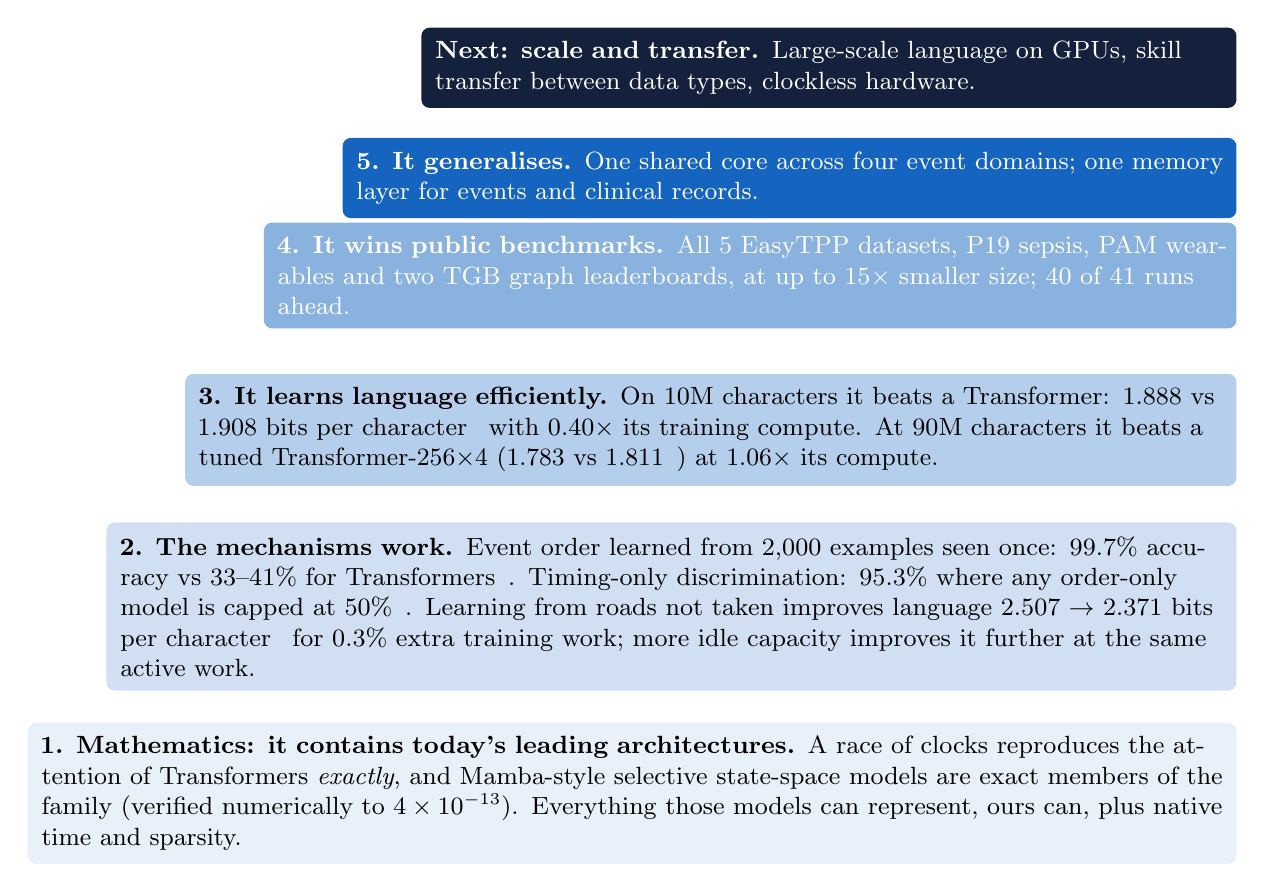
\begin{tikzpicture}[x=1mm,y=1mm,
  step/.style={rounded corners=3pt,text width=#1,align=left,inner sep=5pt,font=\small},
  lab/.style={font=\footnotesize\bfseries,text=white}]
\node[step=150mm,fill=ours!10,anchor=south west] (s1) at (0,0) {\textbf{1. Mathematics: it contains today's leading architectures.} A race of clocks reproduces the attention of Transformers \emph{exactly}, and Mamba-style selective state-space models are exact members of the family (verified numerically to $4\times10^{-13}$). Everything those models can represent, ours can, plus native time and sparsity.};
\node[step=140mm,fill=ours!20,anchor=south west] (s2) at (10,22) {\textbf{2. The mechanisms work.} Event order learned from 2,000 examples seen once: 99.7\% accuracy vs 33--41\% for Transformers \up. Timing-only discrimination: 95.3\% where any order-only model is capped at 50\% \up. Learning from roads not taken improves language 2.507 $\to$ 2.371 bits per character \down{} for 0.3\% extra training work; more idle capacity improves it further at the same active work.};
\node[step=130mm,fill=ours!32,anchor=south west] (s3) at (20,48) {\textbf{3. It learns language efficiently.} On 10M characters it beats a Transformer: 1.888 vs 1.908 bits per character \down{} with 0.40$\times$ its training compute. At 90M characters it beats a tuned Transformer-256$\times$4 (1.783 vs 1.811 \down) at 1.06$\times$ its compute.};
\node[step=120mm,fill=ours!50,anchor=south west,text=white] (s4) at (30,68) {\textbf{4. It wins public benchmarks.} All 5 EasyTPP datasets, P19 sepsis, PAM wearables and two TGB graph leaderboards, at up to 15$\times$ smaller size; 40 of 41 runs ahead.};
\node[step=110mm,fill=ours,anchor=south west,text=white] (s5) at (40,82) {\textbf{5. It generalises.} One shared core across four event domains; one memory layer for events and clinical records.};
\node[step=100mm,fill=ink,anchor=south west,text=white] (s6) at (50,96) {\textbf{Next: scale and transfer.} Large-scale language on GPUs, skill transfer between data types, clockless hardware.};
\end{tikzpicture}
\end{center}

\begin{minipage}[t]{.42\linewidth}\vspace{0pt}
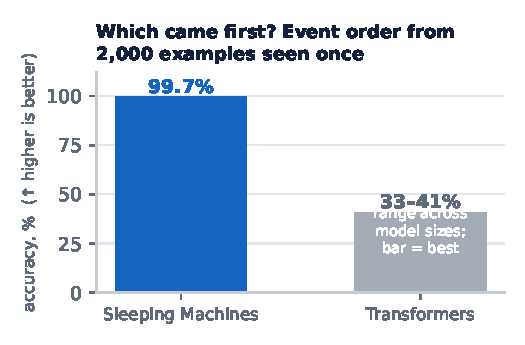
\includegraphics[width=\linewidth]{reasoning.pdf}
\end{minipage}\hfill
\begin{minipage}[t]{.55\linewidth}\vspace{2mm}
\textbf{Why the steps add up.} The family is not a narrow trick for one benchmark. Its mathematics contains the architectures that power today's AI; its mechanisms solve temporal problems those architectures fail at; it already learns language competitively at small scale; and it wins public benchmarks on four kinds of data with one shared memory design. Scale is the remaining work, and each layer beneath it is already demonstrated.

\vspace{2mm}
\textbf{Hardware.} In our cost model, the native language model moves 5.8$\times$ fewer bytes per character than a comparable Transformer at better quality (modelled, not yet measured on silicon; a funded milestone).
\end{minipage}

\newpage
% ---------------------------------------------------------------- rigor
\sect{Rigor}{How we know the results are real}

\begin{minipage}[t]{.485\linewidth}
\begin{tile}[height=31mm]
\textbf{\faLock\ Sealed tests, rules fixed in advance.} Every win uses the benchmark's official data splits. The reporting rule is written down before the test set is touched, and each model is scored on the test set exactly once.
\end{tile}
\begin{tile}[height=31mm]
\textbf{\faRedo\ Independent runs.} Every reported result is the average of independent runs (five seeds or official splits; three pre-registered seeds on TGB), with its spread: 40 of 41 runs are ahead of the best published result.
\end{tile}
\begin{tile}[height=31mm]
\textbf{\faServer\ Reproduced on separate hardware.} The Taxi win was reproduced independently on a separate desktop computer with separately downloaded data: 0.5252 vs 0.5250 nats per event \up, every run above S2P2. One-command kits let third parties rerun the EasyTPP and both TGB wins.
\end{tile}
\end{minipage}\hfill
\begin{minipage}[t]{.485\linewidth}
\begin{tile}[height=31mm]
\textbf{\faCheckDouble\ The benchmark's own scorer agrees.} Re-scoring our models with EasyTPP's own estimation method gives the same results within its sampling noise.
\end{tile}
\begin{tile}[height=31mm]
\textbf{\faSearch\ We found and closed a scoring pitfall.} Timestamps in these datasets are rounded (for example to whole seconds). Flexible models can exploit the rounding for large, fake gains. We built an audit that removes the rounding; we withdrew our own early results that failed it, and every reported win passes it.
\end{tile}
\begin{tile}[height=31mm]
\textbf{\faBalanceScale\ Losses reported as plainly as wins.} Where we are behind, we say so with the numbers and the next test (next page). Comparisons always use the same units and protocol as the published result.
\end{tile}
\end{minipage}

\newpage
% ---------------------------------------------------------------- frontier
\sect{The frontier}{Not ahead yet, or pending, and the next test}

\renewcommand{\arraystretch}{1.35}
{\small
\begin{tabularx}{\linewidth}{>{\bfseries}P{30mm} Y Y}
\toprule
Front & Current result & Next test \\
\midrule
P12 mortality & AUROC 0.871 vs 0.880 \up{} (behind); AUPRC level, 0.585 vs 0.586 \up & Ensemble of five runs, still far smaller than the leader (in progress) \\
Tokenised language (GPT-2 tokens, FineWeb) & Ahead of the classic count model: 6.009 vs 6.537 nats per token \down{} at 1M training tokens (3 runs); at 4M tokens 5.510 vs 6.100, so the lead grows with data; recall across irregular gaps solved (97.5\%) & Further data scaling (16M tokens); a published small Transformer under the same protocol \\
Large-scale language & At 90M characters a tuned Transformer-192$\times$4 leads: 1.704 vs our 1.783 bits per character \down & Race attention at scale on GPU \\
Small-scale language & Tuned small LSTMs lead by 0.04--0.06 bits per character \down{} at 10M characters & Same programme as above \\
Real-world tables & Decision trees lead on the banknote dataset & Learned comparison discovery on real tables \\
FAS v2 (our anonymous-log benchmark) & Level on validation with a time-encoded Transformer reference: 0.702 vs 0.704 AUROC \up{} at about 1/7 of its parameters & Sealed test once the reference seeds finish; a tie is expected under the 0.02 rule \\
Second TPP benchmark (nats per sequence \down) & Wikipedia won; MOOC, Stack Overflow, Github and MIMIC2 behind (page 5); Retweets and LastFM running & Remaining two verdicts; numerically guarded training; a developed attempt with per-sequence type statistics \\
\bottomrule
\end{tabularx}}

\vspace{4mm}
\sect{What comes next}{From proof to platform}
\begin{itemize}
\item \textbf{Publish} the complete event-leaderboard results, after the IP filing decision.
\item \textbf{Scale language}: race attention against competent Transformers at scale on GPUs.
\item \textbf{Transfer}: show that skill learned on one kind of data helps on another.
\item \textbf{First commercial vertical}: event-native models for interleaved, timestamped logs (industry, IoT, IT operations, security, finance) on existing CPUs and GPUs, the shortest path to revenue.
\item \textbf{Hardware}: feasibility on FPGA and neuromorphic silicon for clockless, learning-capable event processors.
\end{itemize}

\begin{callout}
\textbf{The bottom line.} A new model family, designed from first principles around time and sparse events, is already ahead of the best published models on nine public benchmarks across four kinds of data, including every dataset of the field's standard event benchmark, with models up to 15 times smaller, and the same frozen model wins Wikipedia on a second event benchmark without tuning. Its mathematics contains today's dominant architectures. The remaining work is scale, transfer and hardware, and each has a concrete, measurable next step.
\end{callout}

\end{document}
